% Build: latexmk -xelatex paper.tex   (or: make -C paper)
% Every number quoted from an experiment comes from data/numbers.tex, which
% paper/tools/make_data.py derives from the committed evidence logs.
\documentclass[a4paper,11pt]{article}

\usepackage[no-math]{fontspec}
\usepackage{mathpazo}
\setmainfont{TeX Gyre Pagella}
\setsansfont{TeX Gyre Heros}[Scale=MatchLowercase]
\setmonofont{DejaVu Sans Mono}[Scale=0.84]

\usepackage[margin=2.2cm]{geometry}
\usepackage{microtype}
\usepackage{amsmath}
\usepackage{booktabs}
\usepackage{tabularx}
\usepackage{siunitx}
\usepackage{xcolor}
\usepackage{graphicx}
\usepackage{caption}
\usepackage{subcaption}
\usepackage{enumitem}
\usepackage{titlesec}
\usepackage{pgfplots}
\usepgfplotslibrary{groupplots}
\pgfplotsset{compat=1.18}
\usepackage{tikz}
\usetikzlibrary{positioning,fit,arrows.meta,calc}
\usepackage[backend=biber,style=ieee,doi=true,url=false]{biblatex}
\addbibresource{references.bib}
\usepackage[hidelinks]{hyperref}
\hypersetup{pdftitle={Consensus-free task ownership for UAV swarms under partition}, pdfauthor={Charalampos Nadiotis}, pdfsubject={Deterministic simulation and multi-vehicle ArduPilot SITL validation}, pdfkeywords={UAV swarm, task allocation, leases, partition tolerance, ArduPilot, SITL}}
\usepackage[capitalise,noabbrev]{cleveref}

% Generated by paper/tools/make_data.py -- do not edit by hand.
\newcommand{\defaultMission}{17.25}
\newcommand{\jamDetection}{5.00}
\newcommand{\jamMission}{15.50}
\newcommand{\jamPmOwnership}{1.50}
\newcommand{\jamRecovery}{7.25}
\newcommand{\mixBrake}{10.5}
\newcommand{\mixMission}{16.00}
\newcommand{\mixRecovery}{2.25}
\newcommand{\mixSep}{17.0}
\newcommand{\pmDetection}{1.75}
\newcommand{\pmMission}{8.50}
\newcommand{\pmRecovery}{2.50}
\newcommand{\stockBrake}{15.6--17.4}
\newcommand{\stockBrakeDist}{16.9}
\newcommand{\stockBrakeMean}{16.4}
\newcommand{\stockBrakeTime}{4.9}
\newcommand{\stockDrift}{0.60--0.70}
\newcommand{\stockDriftMean}{0.65}
\newcommand{\stockMission}{14.25--14.75}
\newcommand{\stockMissionMean}{14.50}
\newcommand{\stockModelRatio}{1.71}
\newcommand{\stockOvershoot}{0.72}
\newcommand{\stockPass}{3}
\newcommand{\stockRecovery}{7.00--7.25}
\newcommand{\stockRecoveryMean}{7.17}
\newcommand{\stockRuns}{3}
\newcommand{\stockSep}{13.0--14.9}
\newcommand{\stockSepMean}{14.2}
\newcommand{\stockSettle}{11.05}
\newcommand{\stockTuneN}{8}
\newcommand{\tuneTrials}{104}
\newcommand{\tunedBrake}{12.9--13.8}
\newcommand{\tunedBrakeDist}{10.6}
\newcommand{\tunedBrakeMean}{13.2}
\newcommand{\tunedBrakeTime}{2.5}
\newcommand{\tunedDrift}{0.35--0.55}
\newcommand{\tunedDriftMean}{0.45}
\newcommand{\tunedMission}{11.75--12.00}
\newcommand{\tunedMissionMean}{11.92}
\newcommand{\tunedModelRatio}{1.40}
\newcommand{\tunedOvershoot}{0.20}
\newcommand{\tunedPass}{3}
\newcommand{\tunedRecovery}{4.75--5.00}
\newcommand{\tunedRecoveryMean}{4.92}
\newcommand{\tunedRuns}{3}
\newcommand{\tunedSep}{16.4--16.6}
\newcommand{\tunedSepMean}{16.5}
\newcommand{\tunedSettle}{6.10}
\newcommand{\tunedTuneN}{8}


% Colour roles. Vehicles use a validated categorical order; ink is never a series.
\definecolor{uavA}{HTML}{2A78D6}
\definecolor{uavB}{HTML}{EB6834}
\definecolor{uavC}{HTML}{1BAF7A}
\definecolor{uavD}{HTML}{C98500}
\definecolor{ink}{HTML}{1B1B1A}
\definecolor{muted}{HTML}{6B6A65}
\definecolor{faint}{HTML}{D9D8D3}

\titleformat{\section}{\sffamily\large\bfseries}{\thesection}{0.8em}{}
\titleformat{\subsection}{\sffamily\normalsize\bfseries}{\thesubsection}{0.8em}{}
\captionsetup{font=small,labelfont={sf,bf},format=plain}
\setlist{itemsep=2pt,topsep=4pt}
\sisetup{detect-all}
% Monospace names may break after an underscore or a slash.
\newcommand{\code}[1]{\texttt{\codebreaks#1\endcodebreaks}}
\makeatletter
\def\codebreaks{\begingroup\def\_{\textunderscore\allowbreak}\def\/{/\allowbreak}}
\def\endcodebreaks{\endgroup}
\makeatother
\emergencystretch=1.5em

\pgfplotsset{
  paper/.style={
    width=\linewidth, height=5.2cm,
    axis line style={muted}, tick style={muted},
    grid=major, grid style={faint, line width=0.3pt},
    label style={font=\small}, tick label style={font=\footnotesize},
    legend style={font=\footnotesize, draw=none, fill=none},
    every axis plot/.append style={line width=1.1pt},
  },
}

\title{\sffamily\bfseries Consensus-free task ownership for UAV swarms under partition:\\[2pt]
\large deterministic simulation and multi-vehicle ArduPilot software-in-the-loop validation}
\author{Charalampos Nadiotis\\[2pt]\small eudis-swarm project, EUDIS Defence Hackathon 2026, Challenge~2}
\date{October 2026}

\begin{document}
\maketitle

\begin{abstract}
\noindent
A swarm that loses radio contact cannot tell a silent aircraft from a dead one.
We present a coordination scheme in which every UAV acts only on evidence it has
actually received: task ownership is a replicated set of immutable, leased
claims; a peer is declared failed only by a quorum of votes carried over
modelled links; and work held by an aircraft that has gone quiet is recovered
when its lease expires, without any agreement. In a deterministic simulator we
show that this recovery keeps working exactly where consensus cannot: with two
aircraft a loss is undeclarable, yet distributed ownership completes the
mission while a central coordinator never finishes, and across 440 jammed runs
central control failed 68 missions and distributed control none, with
identical failure detection in both. We then drive the same, unchanged
coordination logic with real autopilot firmware: a software-in-the-loop
harness flies four ArduCopter (and mixed ArduCopter/ArduRover) instances in
lock-step with the simulator, commands a physically failed vehicle into a safe
hold, and records a per-step evidence log. In repeated runs every mission
completed, the failed vehicle stopped, its task was recovered by the survivors
and no task ever had two owners. Finally we tune the vehicles' position
controllers by measurement, cutting the mission time from
\stockMissionMean\,\si{s} to \tunedMissionMean\,\si{s} and the recovery after a
failure from \stockRecoveryMean\,\si{s} to \tunedRecoveryMean\,\si{s}. All
results are firmware on simulated airframes; none is a flight result.
\end{abstract}

\section{Introduction}

Contested airspace is not hypothetical. The European Union Aviation Safety
Agency lists the Nicosia flight information region among those affected by GNSS
jamming and spoofing~\cite{easa2026sib}, and a peer-reviewed flight experiment
in that region recorded a receiver losing positioning for most of the time
aloft~\cite{osechas2022gnss}. A swarm operating there must expect its own
links to fail in the same way: partially, intermittently, and with no message
announcing it.

The difficulty is epistemic. When a UAV stops hearing a peer, the peer may be
destroyed, jammed, behind terrain, or briefly out of range and still flying.
Treating silence as failure discards that peer's work and reassigns it, which
duplicates effort whenever the peer was alive. Waiting for certainty is worse:
deciding that a process has failed is a consensus problem, and consensus is
impossible to guarantee under asynchrony with even one faulty
participant~\cite{fischer1985impossibility}. Practical systems escape through
failure detectors that may be wrong~\cite{chandra1996failure}, but a central
reassignment that waits for such a detector inherits its blind spots.

This paper takes the opposite route. Ownership is held through leases~\cite{gray1989leases}
that each UAV's own replica ages on its own clock; a task whose owner has gone
quiet becomes claimable again when the local copy of its lease expires,
whether or not anyone has agreed the owner is gone. Disagreement during a
partition is permitted; the guarantee is that once connectivity is stably
restored every replica converges on one owner per task and the losing
claimant stands down on its own.

\paragraph{Contributions.}
\begin{enumerate}[leftmargin=*]
\item A receiver-local coordination design (\cref{sec:design}) with three
  strictly separated layers, leased immutable claims, quorum-only failure
  declaration and deterministic store-and-forward evidence flooding, enforced
  by tests rather than convention.
\item Deterministic evidence (\cref{sec:sim}) that consensus-free recovery
  survives the conditions that make consensus impossible, in a minimal
  two-aircraft case and in 440-run populations.
\item A firmware-in-the-loop harness (\cref{sec:sitl}) that drives the
  unchanged coordination logic with several ArduPilot~\cite{ardupilot}
  instances: anchored lock-step with measured drift, a one-shot safe-hold
  fail-stop, a shared mission frame, a heterogeneous copter/rover swarm, an
  evidence log and a mechanical pass/fail test card.
\item Repeated SITL missions meeting that card (\cref{sec:results}), and a
  measured tune of the vehicles' position control that shortens missions and
  recovery (\cref{sec:tuning}).
\end{enumerate}

\section{Related work}

Partition-tolerant shared state for robot swarms has been approached through
distributed ledgers: SwarmDAG~\cite{tran2019swarmdag} maintains a
partition-tolerant DAG under extended virtual synchrony. Our goal is narrower
and lighter: one owner per task after healing, with no global log.
Communication-aware allocation~\cite{lu2026commaware} and coverage under
communication constraints~\cite{loizou2016coverage} model links as a planning
constraint; we instead make every decision depend only on what a link actually
delivered. Distributed 3-D search with a varying number of
agents~\cite{papaioannou2023glimpse} addresses joining and leaving agents in
planning; supervisory control theory~\cite{lopes2016supervisory} motivates our
formulation of per-UAV behaviour as composed extended finite-state machines.
Heterogeneous multi-UAV benchmarks such as CARIC~\cite{cao2025caric}
evaluate planning quality; our evaluation is instead about ownership
correctness under loss, and about carrying the same logic onto real autopilot
firmware.

\section{Design}\label{sec:design}

\begin{figure}[t]
\centering
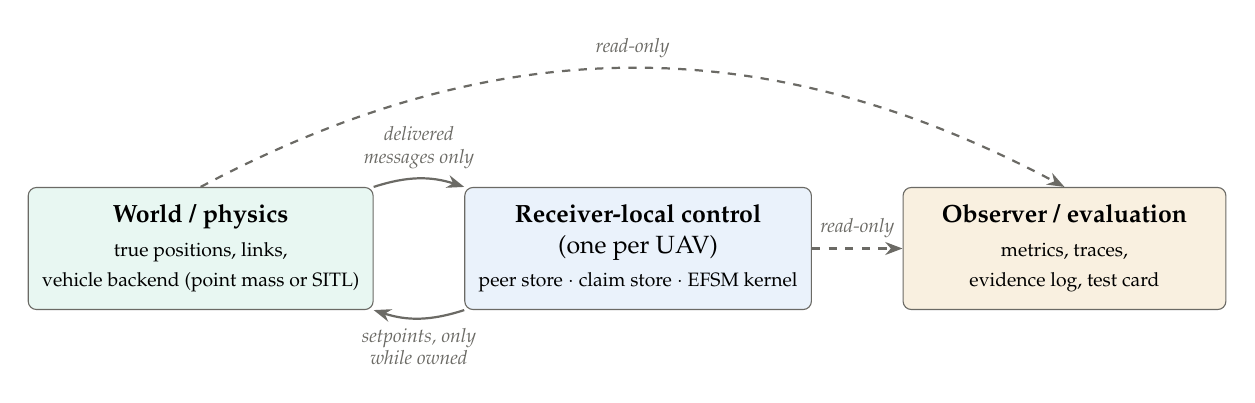
\begin{tikzpicture}[
  layer/.style={draw=muted, rounded corners=3pt, fill=#1, minimum width=4.1cm,
                minimum height=1.55cm, align=center, font=\small, inner sep=5pt},
  arr/.style={-{Stealth[length=2.2mm]}, muted, line width=0.8pt},
  lbl/.style={font=\scriptsize\itshape, text=muted, align=center}]
\node[layer=uavA!10] (ctrl) {\textbf{Receiver-local control}\\(one per UAV)\\[1pt]
  \scriptsize peer store $\cdot$ claim store $\cdot$ EFSM kernel};
\node[layer=uavC!10, left=1.15cm of ctrl] (world) {\textbf{World / physics}\\[1pt]
  \scriptsize true positions, links,\\ \scriptsize vehicle backend (point mass or SITL)};
\node[layer=uavD!12, right=1.15cm of ctrl] (obs) {\textbf{Observer / evaluation}\\[1pt]
  \scriptsize metrics, traces,\\ \scriptsize evidence log, test card};
\draw[arr] (world.north east) to[bend left=18] node[lbl, above]{delivered\\messages only} (ctrl.north west);
\draw[arr] (ctrl.south west) to[bend left=18] node[lbl, below]{setpoints, only\\while owned} (world.south east);
\draw[arr, dashed] (world.north) to[bend left=28] node[lbl, above, pos=0.5]{read-only} (obs.north);
\draw[arr, dashed] (ctrl.east) -- node[lbl, above]{read-only} (obs.west);
\end{tikzpicture}
\caption{The three layers. A UAV's control state is fed only by messages a modelled link delivered;
the observer reads every replica at once (a view no UAV has) and never feeds back.}
\label{fig:layers}
\end{figure}

\paragraph{Layers.} \Cref{fig:layers} shows the load-bearing decision. The
\emph{world} holds true positions and the communication graph; the
\emph{receiver-local control} of each UAV holds its own pose, an immutable task
catalogue, a peer-state store, a claim store and a kernel of composed extended
finite-state machines (contact, peer availability, per-task ownership,
coordination mode); the \emph{observer} computes metrics by reading every
replica at once. No topology fact is ever copied into a UAV's state: a receiver
knows only what it received, and when.

\paragraph{Claims and leases.} Before binding work a UAV publishes an immutable
claim $(\textit{task}, \textit{owner}, \textit{epoch})$. Each replica classifies
a stored claim by its \emph{receiver-local} age $a$: fresh while
$a \le \tau_f$, stale while $\tau_f < a \le \tau_\ell$, expired once $a > \tau_\ell$
(by default $\tau_\ell = \SI{2.5}{s}$ and $\tau_f = \tau_\ell/2$). Stale is not
unclaimed: a replica may create a competing claim only once its own copy has
expired. Epochs are compared only within one owner's stream; reconciliation
supersedes older publications per owner and then picks the lowest validated
owner identifier, so every replica that has seen the same evidence picks the
same winner. A UAV moves toward, renews or completes a task only while its own
replica says it owns it.

\paragraph{Failure is a declaration, not an observation.} Silence, staleness
and unknown state never imply failure. Declaring peer $j$ failed requires votes
from a quorum of $q(N) = \max\bigl(2, \lfloor (N-1)/2 \rfloor + 1\bigr)$
observers, carried over modelled links. One observer can therefore never
declare a peer dead, and a declaration never stops a vehicle: it is evidence,
and first-hand contact from a ``dead'' peer retracts it.

\paragraph{Evidence transport.} Heartbeats are one hop and never forwarded.
Votes, declarations, claims, releases and completion evidence flood the current
connected component by deterministic store-and-forward: stable message and
neighbour order, per-receiver duplicate suppression, no TTL and no random
backoff.

\paragraph{Determinism.} The simulator has no wall-clock time, no unseeded
randomness and no order-dependent iteration; the same command line produces
byte-identical output on any machine. This is what lets exact numbers be
asserted by tests and quoted below.

\section{Deterministic evaluation}\label{sec:sim}

All numbers in this section are evaluator-computed and reproducible from the
commands in \cref{app:repro}; they are taken from the project's measured-results
record.

\paragraph{The quorum floor.} With two aircraft the survivor is the only
observer, so $q(2)=2$ makes the loss undeclarable. Both control modes are then
equally blind; what differs is whether recovery needed the declaration
(\cref{tab:floor}). Central reassignment waits for a declaration that cannot
arrive and holds a task for an aircraft that has stopped; distributed ownership
recovers through lease expiry. A third aircraft restores the quorum and both
modes recover.

\begin{table}[t]
\centering\small
\caption{The quorum floor (\code{demo-quorum-floor} / \code{baseline-quorum-floor}).}
\label{tab:floor}
\begin{tabular}{@{}rlrrll@{}}
\toprule
aircraft & control & declared & never detected & tasks & mission \\
\midrule
2 & central     & 0 & 1 & 2/3 & \textbf{never finishes} \\
2 & distributed & 0 & 1 & 3/3 & completed at \SI{10.75}{s} \\
3 & central     & 1 & 0 & 3/3 & completed \\
3 & distributed & 1 & 0 & 3/3 & completed \\
\bottomrule
\end{tabular}
\end{table}

\paragraph{Populations under jamming.} Across 440 runs (four aircraft, eleven
communication ranges, twenty seeds each, a circular jammer), central control
failed 68 of 220 missions and distributed control none (\cref{fig:range}). A
failed central mission completes 19 of 20 tasks and then burns its
\SI{300}{s} budget holding the last task for an aircraft it cannot reach.
Failure \emph{detection} was identical in both modes at every range (for
example 18/20 seeds undetected at range 50 in both): the two control models
have the same awareness and opposite outcomes.

\begin{figure}[t]
\centering
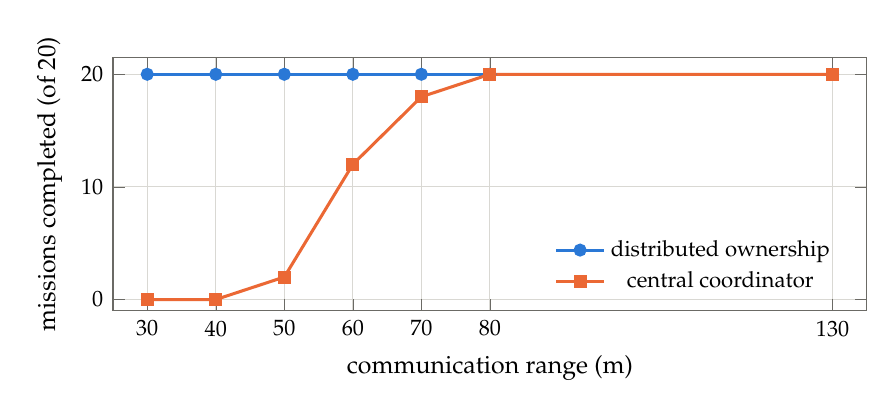
\begin{tikzpicture}
\begin{axis}[paper, height=4.8cm, width=0.92\linewidth,
  xlabel={communication range (m)}, ylabel={missions completed (of 20)},
  ymin=-1, ymax=21.5, xmin=25, xmax=135, xtick={30,40,50,60,70,80,130},
  legend pos=south east]
\addplot[uavA, mark=*, mark size=1.8pt] coordinates {(30,20)(40,20)(50,20)(60,20)(70,20)(80,20)(130,20)};
\addlegendentry{distributed ownership}
\addplot[uavB, mark=square*, mark size=1.8pt] coordinates {(30,0)(40,0)(50,2)(60,12)(70,18)(80,20)(130,20)};
\addlegendentry{central coordinator}
\end{axis}
\end{tikzpicture}
\caption{Missions completed versus communication range under a jammer
(20 seeds per point; ranges 90--120 omitted, all 20/20 in both modes).
Source: measured-results record, section~5.}
\label{fig:range}
\end{figure}

\paragraph{Opposite failure signatures.} With a partition that heals, replicated
ownership strands no work and pays with brief double-booking (0.286
task-seconds on average over 240 runs), while central control strands work it
handed to aircraft it could not reach (4.786 task-seconds on average) and showed
no measured double-booking in that sweep. Neither is better; they are wrong in
different directions, and an operator ``hold'' policy trades 64\,\% of the
double-booking for 59\,\% more mission time.

\section{Firmware in the loop}\label{sec:sitl}

The simulator's motion enters through one interface,
\code{move\_toward(agent, target, elapsed)}. Its default implementation is a
point mass; the SITL backend implements it with a real autopilot. Nothing in
the coordination layer changes, and nothing in the simulator imports the
backend (asserted by test).

\paragraph{Anchored lock-step.} Logical time advances in fixed steps; each
SITL instance free-runs on its own clock. Stepping several instances one after
another lets every clock run on while the others are waited on. The first
version waited until ``last observed time plus the step'', which rounds every
step up to the next telemetry report: on real hardware it ran the vehicle clock
$1.6\times$ ahead of logical time. Each vehicle is now anchored once, all in one
pass after draining the telemetry backlog, and a step waits only until
$t_\text{anchor} + \sum \text{elapsed}$ on that vehicle's own clock. A report is
accepted only if it is strictly newer than the last one, and the residual lead
(drift) is recorded every step. Anchoring cannot slow a fast instance; it makes
the lead visible instead.

\paragraph{Fail-stop.} When the simulator's fault schedule makes an integrated
agent physically non-responsive, the backend sends that vehicle exactly one
safe-hold mode change (ArduCopter \code{BRAKE} or \code{LOITER}, ArduRover
\code{HOLD}) and records whether the autopilot confirmed it. It reads only
physical truth, never the swarm's belief, so a wrongly declared UAV keeps
flying.

\paragraph{Shared frame and deconfliction.} All vehicles report in one local
frame about a shared origin; the launcher starts instance $i$ at its agent's
simulated start position. Copters take off to, and every setpoint holds, their
own altitude band (\SI{20}{m} $+\,5k$); rovers stay on the ground. Separation is
evidenced, not asserted: the log carries each vehicle's observed altitude and
the report gives the minimum pairwise 3-D distance per step.

\paragraph{Evidence and verdict.} Every mission boundary writes one JSON record:
each agent's truth, each live vehicle's observed position, altitude, clock and
drift, every receiver's view of every task, and events including the
fail-stop. The identical configuration is then flown on the point-mass backend
for comparison. A report derives all metrics from the log alone and evaluates a
test card mechanically (\cref{tab:card}).

\begin{table}[t]
\centering\small
\caption{Pass criteria of the multi-vehicle test card (LT3); every run must meet all.}
\label{tab:card}
\begin{tabularx}{\linewidth}{@{}lX@{}}
\toprule
P1 & every task completed and the mission completed \\
P2 & a physical failure, exactly one fail-stop sent to that vehicle, confirmed by the autopilot \\
P3 & the held vehicle actually stopped (final speed below \SI{0.5}{m/s}) \\
P4 & the orphaned work was recovered by the survivors \\
P5 & no concurrent ownership (zero task-seconds with two live owners) \\
P6 & deconfliction held (no step below \SI{5}{m} 3-D separation) \\
P7 & lock-step stayed honest (every vehicle's drift below \SI{1}{s}) \\
P8 & the deterministic comparison run completed \\
\bottomrule
\end{tabularx}
\end{table}

\section{SITL results}\label{sec:results}

\paragraph{Setup.} ArduCopter quad SITL, \code{--speedup 5}, four instances,
eight tasks, UAV~2 physically failed at $t=\SI{4}{s}$, fresh instances for every
run. Runs were made on the team laptop (WSL2, ArduPilot 4.6.0-beta1) and in a
4-vCPU Linux container (ArduPilot 4.8.0-dev, built from source).

\paragraph{Results.} Every container run met every criterion of \cref{tab:card}.
On the laptop, made before the separation metric (P6) existed, three runs completed 8/8 tasks with failure detection at
\SI{1.75}{s}, recovery after the failure in 6.75--\SI{7.25}{s}, maximum drift
0.45--\SI{0.50}{s} and zero concurrent ownership; the braked copter travelled
15.7--\SI{16.5}{m} before coming to rest. In the container, with stock vehicle
parameters (\cref{tab:tune}, stock column), missions took \stockMission\,\si{s} against
\pmMission\,\si{s} for the point-mass run of the same configuration, recovery
took \stockRecovery\,\si{s} (\pmRecovery\,\si{s}), and the minimum separation
never fell below \SI{13}{m}. A mixed swarm of three copters and one rover, with
the rover failed at \SI{8}{s} and held in \code{HOLD}, completed in
\mixMission\,\si{s} with recovery in \mixRecovery\,\si{s}. Under a jammer, live
detection took \jamDetection\,\si{s} and recovery \jamRecovery\,\si{s}, with no
concurrent ownership (the point-mass run of the same configuration showed
\jamPmOwnership\,\si{} task-seconds: a different trajectory through the same
protocol, not an error bar).

\begin{figure}[t]
\centering
\begin{tikzpicture}
\begin{groupplot}[group style={group size=2 by 1, horizontal sep=1.3cm},
  paper, width=0.5\linewidth, height=0.5\linewidth,
  xmin=-2, xmax=104, ymin=-2, ymax=104, axis equal image,
  xlabel={east (m)}, every axis plot/.append style={line width=1.2pt}]
\nextgroupplot[ylabel={north (m)}, title={\small live SITL (ArduCopter)}]
\addplot[only marks, mark=square, mark size=2.2pt, muted, line width=0.6pt] table[x=x,y=y,col sep=comma]{data/tasks.csv};
\addplot[uavA] table[x=x,y=y,col sep=comma]{data/traj_live_1.csv};
\addplot[uavB] table[x=x,y=y,col sep=comma]{data/traj_live_2.csv};
\addplot[uavC] table[x=x,y=y,col sep=comma]{data/traj_live_3.csv};
\addplot[uavD] table[x=x,y=y,col sep=comma]{data/traj_live_4.csv};
\addplot[only marks, mark=x, mark size=4pt, ink, line width=1.2pt] table[x=x,y=y,col sep=comma, restrict expr to domain={\coordindex}{0:0}]{data/failure.csv};
\addplot[only marks, mark=o, mark size=4pt, ink, line width=1pt] table[x=x,y=y,col sep=comma, restrict expr to domain={\coordindex}{1:1}]{data/failure.csv};
\node[font=\scriptsize, anchor=east, ink] at (axis cs:84,22) {UAV\,2 fails};
\node[font=\scriptsize, anchor=east, ink] at (axis cs:77,36) {at rest};
\node[font=\scriptsize, text=uavA] at (axis cs:7,-0.5) {1};
\node[font=\scriptsize, text=uavB] at (axis cs:97,-0.5) {2};
\node[font=\scriptsize, text=uavC] at (axis cs:7,100.5) {3};
\node[font=\scriptsize, text=uavD] at (axis cs:97,100.5) {4};
\nextgroupplot[title={\small point mass, same configuration}]
\addplot[only marks, mark=square, mark size=2.2pt, muted, line width=0.6pt] table[x=x,y=y,col sep=comma]{data/tasks.csv};
\addplot[uavA] table[x=x,y=y,col sep=comma]{data/traj_pm_1.csv};
\addplot[uavB] table[x=x,y=y,col sep=comma]{data/traj_pm_2.csv};
\addplot[uavC] table[x=x,y=y,col sep=comma]{data/traj_pm_3.csv};
\addplot[uavD] table[x=x,y=y,col sep=comma]{data/traj_pm_4.csv};
\node[font=\scriptsize, text=uavA] at (axis cs:7,-0.5) {1};
\node[font=\scriptsize, text=uavB] at (axis cs:97,-0.5) {2};
\node[font=\scriptsize, text=uavC] at (axis cs:7,100.5) {3};
\node[font=\scriptsize, text=uavD] at (axis cs:97,100.5) {4};
\end{groupplot}
\end{tikzpicture}
\caption{One recorded mission (run \code{c5}) seen from above. Left: tracks as each
autopilot reported them, including UAV~2 braking after its fail-stop (\texttimes{} where
it failed, \textopenbullet{} where it came to rest). Right: the point-mass run of the
same configuration, whose failed agent stops dead. Squares are tasks; numbers mark
each vehicle's start.}
\label{fig:tracks}
\end{figure}

\begin{figure}[t]
\centering
\begin{tikzpicture}
\begin{groupplot}[group style={group size=2 by 1, horizontal sep=1.6cm},
  paper, width=0.49\linewidth, height=4.4cm, xlabel={logical time (s)}]
\nextgroupplot[ylabel={observed altitude (m)}, ymin=0, ymax=40, title={\small altitude bands}]
\addplot[uavA] table[x=t,y=alt,col sep=comma]{data/alt_1.csv};
\addplot[uavB] table[x=t,y=alt,col sep=comma]{data/alt_2.csv};
\addplot[uavC] table[x=t,y=alt,col sep=comma]{data/alt_3.csv};
\addplot[uavD] table[x=t,y=alt,col sep=comma]{data/alt_4.csv};
\nextgroupplot[ylabel={drift (s)}, ymin=0, ymax=1.0, title={\small lock-step drift per step}]
\addplot[uavA, only marks, mark size=0.9pt] table[x=t,y=drift,col sep=comma]{data/alt_1.csv};
\addplot[uavB, only marks, mark size=0.9pt] table[x=t,y=drift,col sep=comma]{data/alt_2.csv};
\addplot[uavC, only marks, mark size=0.9pt] table[x=t,y=drift,col sep=comma]{data/alt_3.csv};
\addplot[uavD, only marks, mark size=0.9pt] table[x=t,y=drift,col sep=comma]{data/alt_4.csv};
\addplot[muted, dashed, line width=0.8pt, domain=0:15] {1.0};
\end{groupplot}
\end{tikzpicture}
\caption{The same run: every copter held its own altitude band (UAV~2's band ends at its
failure, after which it is held, not stepped), and the drift of each vehicle's clock ahead
of logical time stayed bounded, well under the \SI{1}{s} limit of criterion P7.}
\label{fig:bands}
\end{figure}

\paragraph{What only the firmware showed.} A braked copter at cruise speed
travels about \SI{16}{m} before it is at rest: the safe hold is a stop
command, not an instantaneous stop, whereas the simulated failed agent stops
dead (\cref{fig:tracks}). The SITL binary exits when its parent process exits,
so the launcher must keep a waiting parent per instance. With several vehicles
a telemetry backlog is the normal case, and reading the head of the queue
presents seconds-old positions as current; the backend drains to the newest
report. And instances do not all run at the speedup requested: under CPU
contention one instance's clock advanced about 17\,\% faster than another's,
which anchoring records as growing drift rather than hiding.

\section{Tuning the vehicles' position control}\label{sec:tuning}

The flights exposed three things the copters' own control did poorly: the
\SI{16}{m} braking distance, legs about $1.7\times$ slower than the point-mass
model, and arrivals that overshot and crept back. All three are ArduCopter
horizontal position control, so we tuned it on the simulated quad by
measurement. Four SITL copters fly, in parallel, four \SI{40}{m} GUIDED steps
and one leg cut by \code{BRAKE} at \SI{8}{m/s} for each candidate parameter set;
trials are scored on settle time (to within \SI{0.3}{m}, staying), overshoot,
final error and braking distance; a candidate that rings, overshoots by more
than \SI{1.5}{m}, strays in altitude or rebounds after braking is disqualified
outright. A staged coordinate search over safety-bounded values ran
\tuneTrials{} trials; the winner was then flown \tunedTuneN{} times against
\stockTuneN{} flights of the stock parameters (\cref{tab:tune}, \cref{fig:step}).
The inner attitude-rate loops were not touched. This is a tune of the
simulated quad, not of any aircraft.

\begin{table}[t]
\centering\small
\caption{Position-control tune: confirmation flights (top) and the LT3 mission (bottom).}
\label{tab:tune}
\begin{tabular}{@{}lrr@{}}
\toprule
& stock & tuned \\
\midrule
settle time, \SI{40}{m} step & \stockSettle\,\si{s} & \tunedSettle\,\si{s} \\
overshoot & \stockOvershoot\,\si{m} & \tunedOvershoot\,\si{m} \\
\code{BRAKE} from about \SI{8}{m/s} & \stockBrakeDist\,\si{m} & \tunedBrakeDist\,\si{m} \\
\midrule
mission time (3 runs) & \stockMission\,\si{s} & \tunedMission\,\si{s} \\
recovery after the failure & \stockRecovery\,\si{s} & \tunedRecovery\,\si{s} \\
distance travelled after the fail-stop & \stockBrake\,\si{m} & \tunedBrake\,\si{m} \\
minimum 3-D separation & \stockSep\,\si{m} & \tunedSep\,\si{m} \\
live / point-mass mission time & \stockModelRatio & \tunedModelRatio \\
test card & \stockPass/\stockRuns{} pass & \tunedPass/\tunedRuns{} pass \\
\bottomrule
\end{tabular}
\\[4pt]\parbox{0.8\linewidth}{\centering\footnotesize Changed: \code{PSC\_NE\_POS\_P} $1\to2$,
\code{PSC\_NE\_VEL\_I} $1\to1.5$, \code{PSC\_NE\_JERK} $5\to10$,\\ \code{WP\_ACC} $2.5\to5$,
\code{ATC\_ANGLE\_MAX} $30\to35$ (\code{config/sitl/copter-tuned.parm}).}
\end{table}

\begin{figure}[t]
\centering
\begin{tikzpicture}
\begin{groupplot}[group style={group size=2 by 1, horizontal sep=1.6cm},
  paper, width=0.49\linewidth, height=4.6cm]
\nextgroupplot[xlabel={time after the command (s)}, ylabel={along-track position (m)},
  xmin=4, xmax=14, ymin=36, ymax=41.2, title={\small \SI{40}{m} GUIDED step},
  legend pos=south east]
\addplot[muted, dashed, line width=0.8pt, domain=4:14, forget plot] {40};
\addplot[uavB] table[x=t,y=along,col sep=comma]{data/step_stock.csv};
\addlegendentry{stock}
\addplot[uavA] table[x=t,y=along,col sep=comma]{data/step_tuned.csv};
\addlegendentry{tuned}
\nextgroupplot[xlabel={time after \code{BRAKE} (s)}, ylabel={ground speed (m/s)},
  xmin=-0.5, xmax=6, ymin=0, ymax=9, title={\small \code{BRAKE} from \SI{8}{m/s}},
  legend pos=north east]
\addplot[uavB] table[x=t,y=speed,col sep=comma]{data/brake_stock.csv};
\addlegendentry{stock}
\addplot[uavA] table[x=t,y=speed,col sep=comma]{data/brake_tuned.csv};
\addlegendentry{tuned}
\end{groupplot}
\end{tikzpicture}
\caption{Step and braking response on the SITL quad, stock versus tuned (one recorded
flight each). The stock controller overshoots and creeps back; the tuned one settles
sooner. Under \code{BRAKE}, deceleration builds faster with the higher jerk limit.}
\label{fig:step}
\end{figure}

The search also mapped the boundaries. Doubling the position gain was the
largest single gain; lowering the velocity gain or removing its derivative
term made the vehicle ring; doubling the braking jerk again made it rebound by
more than a metre after stopping. A tighter arrival tolerance did \emph{not}
shorten missions, because a task completes the first time a vehicle passes
within the tolerance on the way in, so overshoot never delays completion;
mission time is set by acceleration. The braking gain is smaller in the mission
than in the fixed-speed test because the tuned copters are faster when they
fail. The harness itself needed one correction: ArduCopter reads its leg
acceleration limits only when GUIDED initialises, and re-selecting GUIDED while
in it is a no-op, so early shaping trials flew with the previous candidate's
limits; trials now pass through \code{BRAKE} first and that stage was re-flown.

\section{Limitations and readiness}

\begin{itemize}[leftmargin=*]
\item \textbf{Not flight.} SITL runs real autopilot firmware on a simulated
  airframe. No physical flight has been performed, and the tuned parameters
  must never be flown on a real aircraft.
\item \textbf{Modelled radio.} The links, the jammer and the failure are the
  simulator's models; the radio model is an analytical abstraction, not
  calibrated RF.
\item \textbf{Non-reproducible live numbers.} SITL runs vary between runs and
  machines; they are reported as ranges and never as deterministic results.
\item \textbf{Limited generality.} One main scenario family (four aircraft, a
  \SI{100}{m} square, one jammer) plus a two-aircraft counterexample and a
  small fleet comparison.
\item \textbf{Lock-step, not free-running.} Logical time is stepped against
  each vehicle's clock; a free-running integration remains future work.
\end{itemize}

Against the usual readiness scale~\cite{ec2014trl}, the coordination function is
validated in simulation (TRL\,3). The multi-vehicle SITL test (LT3) passed on
two machines with a mechanical verdict; a TRL\,4 claim for the coordination
function additionally requires the protocol to run as separate processes over
a real network that is partitioned and healed (LT5), which is not reported here.

\section{Conclusion}

Making every decision depend only on evidence a UAV actually received, holding
ownership through leases that each replica ages on its own clock, and refusing
to equate silence with failure gives a swarm that keeps completing its mission
exactly where agreement is impossible. The same logic, unchanged, has driven
four real autopilots through a mission in which one vehicle was physically
stopped and its work was taken over by the others, and every container run
passed a mechanical test card. What remains between this and a field claim is a real
network, real radios and real airframes.

\printbibliography

\appendix
\section{Reproducing the results}\label{app:repro}
\begin{small}
\begin{verbatim}
# deterministic results (any machine, byte-identical)
eudis-swarm --scenario demo-quorum-floor
eudis-swarm --scenario baseline-quorum-floor
eudis-swarm-sweep --param communication-range --from 30 --to 130 --steps 11 \
  --seeds 20 --jammer 40,50,15,3,8 --task-control distributed --output d.csv

# multi-vehicle SITL test card (ArduPilot built: ./waf copter rover)
scripts/sitl-lt3.sh 3 5                                  # stock vehicles
COPTER_PARAMS=config/sitl/copter-tuned.parm scripts/sitl-lt3.sh 3 5
python scripts/sitl_swarm_report.py --check lt3-*/run*.jsonl

# the position-control tune
scripts/sitl-swarm.sh 4 5 && python scripts/sitl_tune.py --workers 4

# this paper: data from the committed logs, then XeLaTeX
python paper/tools/make_data.py && make -C paper
\end{verbatim}
\end{small}
The evidence logs behind \cref{sec:results,sec:tuning} are committed under
\code{docs\/data\/sitl/}, and \code{paper\/tools\/make\_data.py} recomputes every
number quoted from them.

\end{document}
